\documentclass[11pt,a4paper]{article}
\usepackage{a4wide}
\usepackage[utf8]{inputenc}
\usepackage[T2A]{fontenc}
\usepackage{graphics,graphicx,epsfig}
\usepackage{amssymb,amsfonts,amsthm,amsmath,mathtext,cite,enumerate,float}
\usepackage[english,russian]{babel}
\usepackage[all]{xy}
\usepackage{morefloats}
\usepackage{pgf}
\usepackage[debug,outputdir={docgraphs/}]{dot2texi}
\usepackage{tikz}
\usepackage{scalefnt}
\usepackage{listings}
\usepackage{float}
\usepackage{verbatim}
\usepackage{placeins}
\usepackage{url}
\usepackage{babelbib}
\usepackage{pbox}
\usepackage{grffile}
\usepackage{color}
\usepackage{xfrac}
\usepackage{comment}
\usepackage{rotating}
\usetikzlibrary{shapes,arrows}
\usetikzlibrary{decorations.pathmorphing}

% Comment the following block when compiling this .tex with a saner compiler than texlive.
\makeatletter
\def\@settitle{\begin{center}%
    \baselineskip14\p@\relax
    \bfseries
    \@title
  \end{center}%
}

%\renewcommand{\section}{\@startsection {section}{1}%
%  \z@{.7\linespacing\@plus\linespacing}{.5\linespacing}%
%  {\normalfont}}
%\renewcommand{\section}{\@startsection {section}{1}
%  \z@{2.7ex \@plus 1ex}{1.0ex}%
%  {\normalfont}}
\makeatother

\theoremstyle{definition}
\newtheorem{algo}{Алгоритм}
\newtheorem{theorem}{Теорема}
\newtheorem{stat}{Утверждение}
\newtheorem{defin}{Определение}
\newtheorem{note}{Замечание}

\begin{document}

\begin{center}
  О ВОЗМОЖНОСТИ ПРИМЕНЕНИЯ МЕТОДОВ МОНТЕ-КАРЛО В АНАЛИЗЕ НЕЛИНЕЙНЫХ РЕГРЕССИОННЫХ МОДЕЛЕЙ

  \bigskip
  Г.\,И.~Рудой
\end{center}

\section*{Введение}

Символьная регрессия часто используется для построения экспертно
интерпретируемых моделей
\cite{davidson:2000:snrea,reference/ml/X10vc,StrijovW10,Strijov08InductMethods,Rudoy13}.
В приложении к естественнонаучным
экспериментам речь идет о восстановлении функциональной зависимости
между измеряемыми и задаваемыми с некоторой точностью параметрами,
как то: зависимость термоэмиссионного тока
электронной лампы от температуры катода $I_k(T)$ при неизменных геометрии
системы и разности потенциалов, зависимость мощности излучения
непрерывного лазера от коэффициента отражения выходного зеркала $W_l(R)$
при постоянных модовой структуре излучения и мощности возбуждения
активной среды, зависимость показателя преломления материала от длины
волны $n(\lambda)$ при постоянной температуре и т.~п., далее мы более подробно
рассмотрим именно последний случай.

При регрессионном анализе такого рода экспериментов необходимо
учитывать следующие обстоятельства:
\begin{enumerate}
  \item Все измеряемые (и контролируемые) параметры в каждой
	экспериментальной точке определяются с некоторой (обычно известной) 
	точностью, причем абсолютная погрешность $\sigma_i$ соответствующего параметра может
	существенно изменяться в исследуемом диапазоне. Например, если в качестве
	спектрального прибора, выделяющего конкретную длину волны $\lambda_i$ при
	измерении $n_i(\lambda_i)$, используется дифракционная решетка, то
	$\frac{\sigma_i}{\lambda_i} \approx \text{const}$, и
	считать погрешность определения длины волны постоянной некорректно для
	измерений в достаточно широком спектральном дипазоне.
  \item Как правило, эксперимент ставится так, что измеряется функциональная
	зависимость от одной переменной $х$, то есть, строится зависимость вида $y(x,
	\boldsymbol{\omega})$, где $\boldsymbol{\omega}$~--- набор параметров,
	которые поддерживаются неизменными. Как
	отмечалось выше, параметры поддерживаются постоянными с конечной
	точностью и в ряде случаев при построении модели это обстоятельство 
	необходимо учитывать. Однако обычно эксперт заранее может оценить
	влияние вариаций условий эксперимента и обеспечить необходимую
	стабильность проведения измерений. В противном случае необходимо прямо
	учитывать зависимость измеряемой характеристики от нескольких
	переменных, что для целей настоящей работы непринципиально.
  \item В большинстве случаев эксперт заранее знает вид
	искомой функциональной зависимости, или же требуется провести выбор
	между несколькими возможными вариантами, что упрощает задачу регрессии.
	В то же время для эксперта важнейшее значение имеет не только
	определение оптимальных численных коэффициентов регрессионной
	формулы путем минимизации некоторого функционала, но и дисперсия
	указанных коэффициентов и, что предпочтительнее, связь дисперсии
	регрессионных коэффициентов с точностью определения измеряемых
	(контролируемых) в эксперименте величин. Это особенно существенно в тех
	случаях, когда коэффициенты регрессионной модели прямо связаны с
	фундаментальными характеристиками исследуемого процесса и по ним
	рассчитывается, например эффективная масса электронов в полупроводнике,
	температура Дебая, резонансная частота и затухание оптического перехода и
	т.~д.~--- соответственно, точность измерения соответствующих материальных
	констант определяется точностью вычисления коэффициентов регрессионной
	модели.
\end{enumerate}

В такой постановке, когда требуется определить не только
оптимальные коэффициенты регрессионной модели, но и их погрешность, насколько нам
известно, задача нелинейной регрессии не рассматривалась. Известны
теоретические результаты для случая линейной регрессии:
\[
  y = ax + b,
\]
в случае, когда дисперсия всех экспериментально измеренных значений $y_i$
зависимой переменной $y$ одна и та же $D(y_i) = \sigma^2$, а значения независимой
переменной $x_i$ известны точно: $D(x) = 0$. Тогда при переходе к представлению
\[
  y_i = a(x_i - \overline{x}) + b + \xi_i \mid i \in \{ 1, \dots, n \},
\]
где $\overline{x} = \frac{\sum_{i = 1}^n x_i}{n}$, согласно \cite{Vatunin05}, случайные величины $a$ и $b$ независимы
и нормально распределены, и, кроме того, их дисперсии выражаются известными соотношениями:
\begin{equation}
  \label{eq:classic_da}
  D(a) = \frac{\sigma^2}{\sum_{i = 1}^n (x_i - \overline{x})^2}.
\end{equation}
\begin{equation}
  \label{eq:classic_db}
  D(b) = \frac{\sigma^2}{n}.
\end{equation}

В настоящей работе предложен общий метод определения
погрешности коэффициентов нелинейной регрессии, и на примере зависимости
$n(\lambda)$ для прозрачного полимера определена зависимость погрешности
параметров регрессии от точности определения длины волны и показателя
преломления прозрачного полимера. Здесь мы ограничиваемся одной
независимой переменной $\lambda$. Обобщение предлагаемого метода на случай
нескольких переменных проводится очевидным образом.

\section{Основная гипотеза}

Пусть имеется обучающая выборка $(x_i, y_i) \mid i = \{ 1, \dots, n \}$,
причем для каждого значения $x_i, y_i$ известно распределение вероятности отклонения
независимой и зависимой переменных от их среднего значения $P_i^x(x - x_i)$ и
$P_i^y (y - y_i)$ соответственно, которые обычно принимаются гауссовыми и для которых
считаются известными значения дисперсий $\sigma_i^x$, $\sigma_i^y$.

Пусть далее с помощью некоторого алгоритма регрессии строится
зависимость $y(x, \boldsymbol{\omega})$, минимизирующая некоторый функционал S,
например среднеквадратичное отклонение:
\begin{equation}
  S = \sum_{i=1}^n \big(y (x_i, \boldsymbol{\omega}) - y_i\big)^2 \underset{\boldsymbol{\omega}}{\rightarrow} \min.
  \label{eq:S}
\end{equation}
Для таким образом определенного функционала, а также для его модификаций,
учитывающих сложность регрессионной модели \cite{Rudoy13}, процедура минимизации эффективно
проводится спомощью алгоритма Левенберга-Марквардта (АЛМ) \cite{Marquardt1963Algorithm,more:78}.

Далее фиксируем структурный вид полученной зависимости $y(x, \boldsymbol{\omega})$ и
многократно повторяем следующую вычислительную процедуру:
\begin{enumerate}
  \item На $k$-м шаге генерируется случайная выборка $(x_i^k, y_i^k)$, при этом
	вероятность появления в выборке значения $x_i^k$ пропорциональна
	$P_i^x (x_i^k - x_i)$, а вероятность появления $y_i^k$ аналогично
	пропорциональна $P_i^y (y_i^k - y_i)$.
  \item Для таким образом построенной реализации набора экспериментальных
    данных $(x_i^k, y_i^k)$ (далее~--- реализация), используя один и тот же
    алгоритм оптимизации, находим оптимальный (минимизирующий выбранный
	функционал) набор $\boldsymbol{\omega}_k$ коэффициентов регрессии
	$y(x, \boldsymbol{\omega})$ для $k$-й реализации.

	Таким образом, для каждого конкретного коэффициента регрессии
	$\boldsymbol{\omega}_p$ получаем совокупность его значений в сгенерированных реализациях
	$\{ \boldsymbol{\omega}_p^k \}$.
  \item Для достаточно большого числа реализаций $M$ стандартно определим
	  среднее значение и стандартное отклонение соответствующего
	  коэффициента регрессии $\boldsymbol{\omega}_p$:
	  \begin{equation}
		\label{eq:omega_mean}
		\overline{\boldsymbol{\omega}_p} = \sum_{i = 1}^M \boldsymbol{\omega}_p^k,
	  \end{equation}
	  \begin{equation}
		\label{eq:omega_stddev}
		D(\boldsymbol{\omega}_p) = \sqrt{\frac{1}{M - 1} \sum_{i = 1}^M (\boldsymbol{\omega}_p^k - \overline{\boldsymbol{\omega}_p})}.
	  \end{equation}
\end{enumerate}

Наша гипотеза состоит в том, что полученные согласно \eqref{eq:omega_mean} и \eqref{eq:omega_stddev}
значения соответствуют реальности. Предлагаемый подход к определению
погрешности регрессионных коэффициентов, очевидно, представляет собой
фактически применение метода типа Монте-Карло к задаче регрессии.

Из предложенной интерпретации также следует очевидный критерий
останова вычислительной процедуры, когда с ростом числа реализаций $М$
вариация значений $\overline{\boldsymbol{\omega}_p}$ и
$D(\boldsymbol{\omega}_p)$ становится меньше экспертно выбранного
значения.

Необходимо заметить, что в общем случае пределы выражений типа
\eqref{eq:omega_mean} и \eqref{eq:omega_stddev}
при $M \rightarrow \infty$ могут и не существовать, что делает предложенную
вычислительную схему некорректной. Однако для достаточно гладких
функций, которые собственно и представляют практический интерес,
корректность предложенной процедуры можно строго доказать, что, однако,
выходит за рамки данной работы.

\section{Модельный случай}

Определим предложенным в предыдущей части методом дисперсию коэффициентов
линейной регрессии $y = kx + b \mid k = 3, b = 10$, независимая
переменная $x$ определена точно, а погрешность зависимой переменной $y$
постоянна и имеет гауссово распределение. Независимая переменная
определена в 10 (30, 50) точках отрезка $[0, 10]$, количество реализаций
составляло 10 миллионов, оптимизация регрессии проводилось с помощью АЛМ.

\begin{figure}[h]
  \centering
  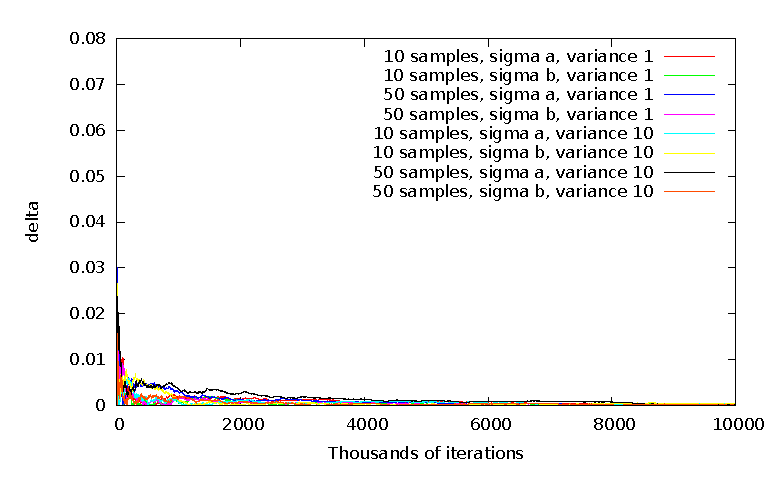
\includegraphics[scale=1.2]{figs/classic/variance_all_0_all.eps}
  \caption{График зависимости $\delta$ от числа итераций (от 0 до $10^7$ итераций).}
  \label{fig:classic_all_0_all}
\end{figure}

\begin{figure}[h]
  \centering
  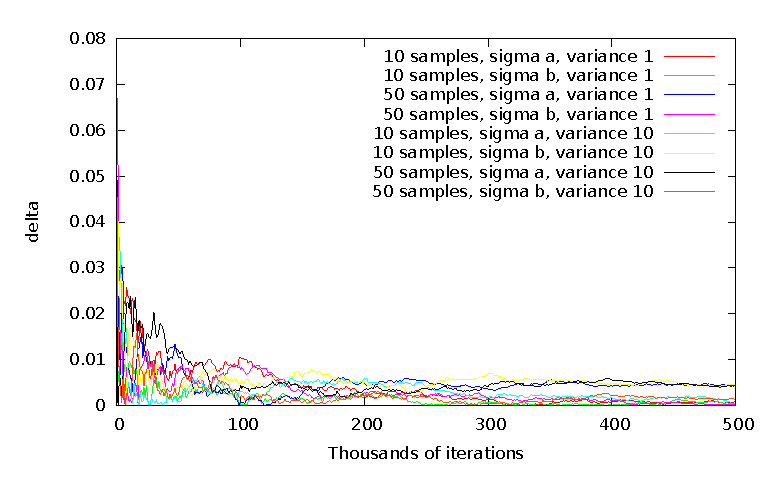
\includegraphics[scale=1.2]{figs/classic/variance_all_0_500.eps}
  \caption{График зависимости $\delta$ от числа итераций (от 0 до $5 \cdot 10^5$ итераций).}
  \label{fig:classic_all_0_500}
\end{figure}

\begin{figure}[h]
  \centering
  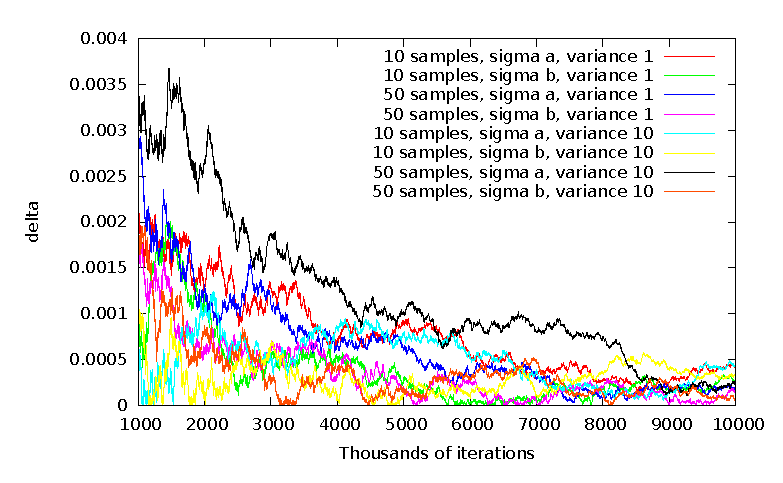
\includegraphics[scale=1.2]{figs/classic/variance_all_1000_all.eps}
  \caption{График зависимости $\delta$ от числа итераций (от $10^6$ до $10^7$ итераций).}
  \label{fig:classic_all_1000_all}
\end{figure}

На рис. \ref{fig:classic_all_0_all}-\ref{fig:classic_all_1000_all}
по оси абсцисс указано количество реализаций $M$, а по
оси ординат для каждого из коэффициентов $k$, $b$ отношение
$\frac{\sigma_{c.e.} - \sigma_t}{\sigma_t}$, где $\sigma_{c.e.}$~---
значение дисперсии, полученное в вычислительном эксперименте, а
$\sigma_{t}$~--- точное теоретическое значение дисперсии согласно 
\eqref{eq:classic_da} \eqref{eq:classic_db}.

Как видно, для $M \approx 107$ относительное различие $\frac{\sigma_{c.e.} - \sigma_t}{\sigma_t}$ не
превышает $0.05 \%$, что на наш взгляд является хорошим результатом и
свидетельствует в пользу корректности обсуждаемого подхода и основной
гипотезы.

\FloatBarrier

\bibliographystyle{babunsrt-lf}
%\bibliographystyle{babunsrt}
%\bibliographystyle{unsrt}
\bibliography{bibliography}

\end{document}
